% ============================================================
%  SECTION 3 — Introduction to Quantum Computing
% ============================================================
\section{Introduction to the World of Quantum Computing}

\begin{smjnote}
Our goal in this article is not to focus on quantum computing, there are
multiple lectures about it, and some really advanced topics will be needed
during section 4.3 to explain the implementation of Shor's algorithm, and
these concepts need their own article. If you feel a bit lost during the
quantum computing parts, this is totally normal, but I am going to do my best
to keep you on board.
\end{smjnote}

\begin{smjnote}
While reading this article, you may encounter some intermediary algorithms,
while the article will still give a short explanation of them, again our goal
won't be to go deeply into them. If you would like to know more about them,
a quick Google search will serve you.
\end{smjnote}

\subsection{The Mathematics of Quantum States}

Before diving into quantum computing, let us start from familiar ground. A
classical computer processes information using \textbf{bits} --- the smallest
unit of information, which can take one of two values: $0$ or $1$. These bits
are physically realized through the presence or absence of electrical signals.
A classical register is simply a collection of bits, and all classical
computation reduces to manipulating these $0$s and $1$s through logical
operations.

Quantum computing builds on this foundation but introduces a fundamentally
different model of information. Instead of bits, it uses \textbf{quantum
bits}, or \textbf{qubits}.

We have all heard this, without really getting what is happening behind it.
We also heard the famous sentence: While bits must be either in a $0$ or $1$
state, a qubit can be in a superposition of states $\ket{0}$ and $\ket{1}$.
Some people also heard that when you measure a quantum state, you can't
measure the superposition, you just randomly measure one of the possible
states. At measurement, you can say that the quantum states collapse into
exactly one. Let's try to discover what is really happening behind the scenes.

Formally, a quantum state (for the sake of the understanding we will first
define a quantum state made by only 1 qubit; so a state ``between'' the
$\ket{0}$ and the $\ket{1}$) is described by amplitudes $\alpha$ and $\beta$
(where $\alpha, \beta \in \mathbb{C}$), with probability $|\alpha|^2$ of
measuring 0, and probability $|\beta|^2$ of measuring 1. Thus, we have:
$$
|\alpha|^2 + |\beta|^2 = 1
$$
The randomness is indeed real. But it is not uniform as many people would
think, it is explicitly governed by $\alpha$ and $\beta$.
And we write for a state $X$:
$$
\ket{X} = \alpha \ket{0} + \beta \ket{1}
$$
For a state with 2 qubits, instead of 1, we get $2^2$ possibilities:
$$
\ket{X} = \alpha \ket{00} + \beta \ket{01} + \gamma \ket{10} + \delta \ket{11}
$$
$$
|\alpha|^2 + |\beta|^2 + |\gamma|^2 + |\delta|^2 = 1
$$
As an example, consider the state $Y$ where:
$$
\ket{Y} = \frac{1}{2} \ket{00} + \frac{1}{2} \ket{01} + \frac{1}{2} \ket{10}
+ \frac{1}{2} \ket{11}
$$
If we try to measure the state $Y$, we have equally $\frac{1}{4}$ probability
of measuring either $00$, $01$, $10$, or $11$.

Now, a more sophisticated way to define quantum states is by looking at them
as elements of the unit sphere (since $|\alpha|^2 + |\beta|^2 = 1$) of a
vector space.
Indeed, one can notice that for a state made by one qubit, it is basically a
vector of $\mathbb{C}^2$, that has basis $\{\ket{0}, \ket{1}\}$.
If we take the previous quantum state we mentioned, it would correspond to the
following vector:

\begin{center}
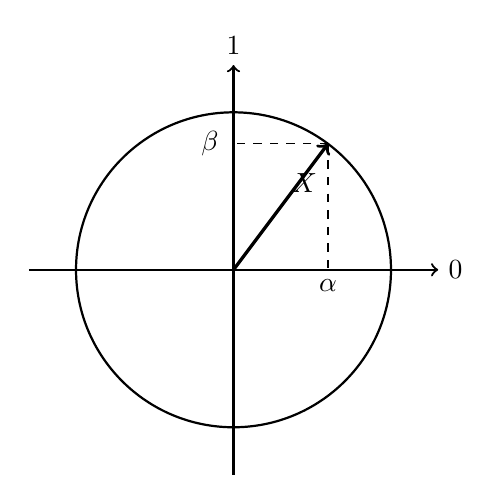
\begin{tikzpicture}[scale=2]
    \draw[black, thick] (0,0) circle (1);
    \draw[black, thick, ->] (-1.3,0) -- (1.3,0) node[right] {$\ket{0}$};
    \draw[black, thick, ->] (0,-1.3) -- (0,1.3) node[above] {$\ket{1}$};
    \draw[black, very thick, ->] (0,0) -- (0.6,0.8);
    \draw[black, dashed] (0.6,0.8) -- (0.6,0);
    \draw[black, dashed] (0.6,0.8) -- (0,0.8);
    \node[black] at (0.6,-0.1) {$\alpha$};
    \node[black] at (-0.15,0.8) {$\beta$};
    \node[black] at (0.45,0.55) {$\ket{X}$};
\end{tikzpicture}\\
$\ket{X} = \alpha \ket{0} + \beta \ket{1} \  := \
\begin{bmatrix} \alpha \\ \beta \end{bmatrix}$
\end{center}

For a quantum state made by two qubits, the vector would live in
$\mathbb{C}^2 \otimes \mathbb{C}^2$, with basis
$\{\ket{00}, \ket{01}, \ket{10}, \ket{11}\}$.
$$
\ket{X} = \alpha \ket{00} + \beta \ket{01} + \gamma \ket{10} + \delta \ket{11}
\ := \ \begin{bmatrix} \alpha \\ \beta \\ \gamma \\ \delta \end{bmatrix}
$$
In general, a system of $n$ qubits lives in the space
$(\mathbb{C}^2)^{\otimes n}$, which has dimension $2^n$.

\begin{smjnote}
The symbol $\otimes$ denotes the tensor product. On the surface, it looks
similar to the Cartesian product: both produce ordered pairs. However, they
differ in how scalar multiplication and addition behave.

In $X \times Y$:
\begin{itemize}
    \item $c(x, y) = (cx, cy)$
    \item $(x, y) + (w, z) = (x+w, y+z)$
\end{itemize}
In $X \otimes Y$:
\begin{itemize}
    \item $c(x \otimes y) = cx \otimes y = x \otimes cy$
    \item $(x + w) \otimes y = x \otimes y + w \otimes y$
    \item $x \otimes (y + z) = x \otimes y + x \otimes z$
\end{itemize}
As a consequence, elements like $x \otimes y + w \otimes z$ cannot be
simplified further --- and these are precisely the entangled states.
\end{smjnote}

Now that we have established that quantum states are vectors living in
$(\mathbb{C}^2)^{\otimes n}$, it is natural to ask: how do we transform them?
The answer is through linear maps on these vector spaces, represented as
matrices. In the quantum computing world, we call these \textbf{quantum gates}.

\begin{smjdefinition}
A \textbf{quantum gate} is a unitary operator acting on
$(\mathbb{C}^2)^{\otimes n}$. Every quantum gate must be represented by a
unitary matrix $U$, meaning its conjugate transpose satisfies $U^\dagger U = I$.
\end{smjdefinition}

The unitarity condition is not arbitrary --- it ensures that quantum gates are
reversible, and that they preserve the normalization condition
$|\alpha|^2 + |\beta|^2 = 1$: a valid quantum state must remain a valid
quantum state after a transformation.

A simple first example is the \textbf{Pauli-X gate}, the quantum analogue of
a classical NOT gate. It simply flips $\ket{0}$ to $\ket{1}$ and $\ket{1}$
to $\ket{0}$:
$$
X = \begin{bmatrix} 0 & 1 \\ 1 & 0 \end{bmatrix}
$$
$$
X\ket{0} = \begin{bmatrix} 0 & 1 \\ 1 & 0 \end{bmatrix}
\begin{bmatrix} 1 \\ 0 \end{bmatrix} = \begin{bmatrix} 0 \\ 1 \end{bmatrix}
= \ket{1}, \qquad
X\ket{1} = \begin{bmatrix} 0 & 1 \\ 1 & 0 \end{bmatrix}
\begin{bmatrix} 0 \\ 1 \end{bmatrix} = \begin{bmatrix} 1 \\ 0 \end{bmatrix}
= \ket{0}
$$
You can verify that $X^\dagger X = I$, confirming it is indeed unitary. With
this foundation, we are ready to look at a less trivial --- and far more
powerful --- gate: the Hadamard gate, which we will encounter in section 4.

\subsection{From Theory to Hardware: Building a Qubit}

The physical implementation of qubits is a deep topic in its own right, and
going into full detail would take us far from the scope of this article. That
said, to give the reader a sense of grounding, we briefly sketch one of the
most common approaches.

So how do we create such a computer? How do we create a qubit? Usually in a
classical computer, a bit of $0$ or $1$ is created by using the ``presence''
or ``absence'' of electricity, but we cannot do it for quantum computers ---
there is no ``electricity a bit present or a bit absent''.

We had to find a new way to describe the $0$ and the $1$ state.

A widely used method to build qubits is by using the \textbf{spin of an
electron}, often the electron of a phosphorus atom embedded in silicon. The
two possible spin orientations --- \textbf{spin-up} and \textbf{spin-down}
--- are used to represent the states $\ket{1}$ and $\ket{0}$ respectively.

\begin{figure}[ht]
    \centering
    \begin{minipage}{0.45\textwidth}
        \centering
        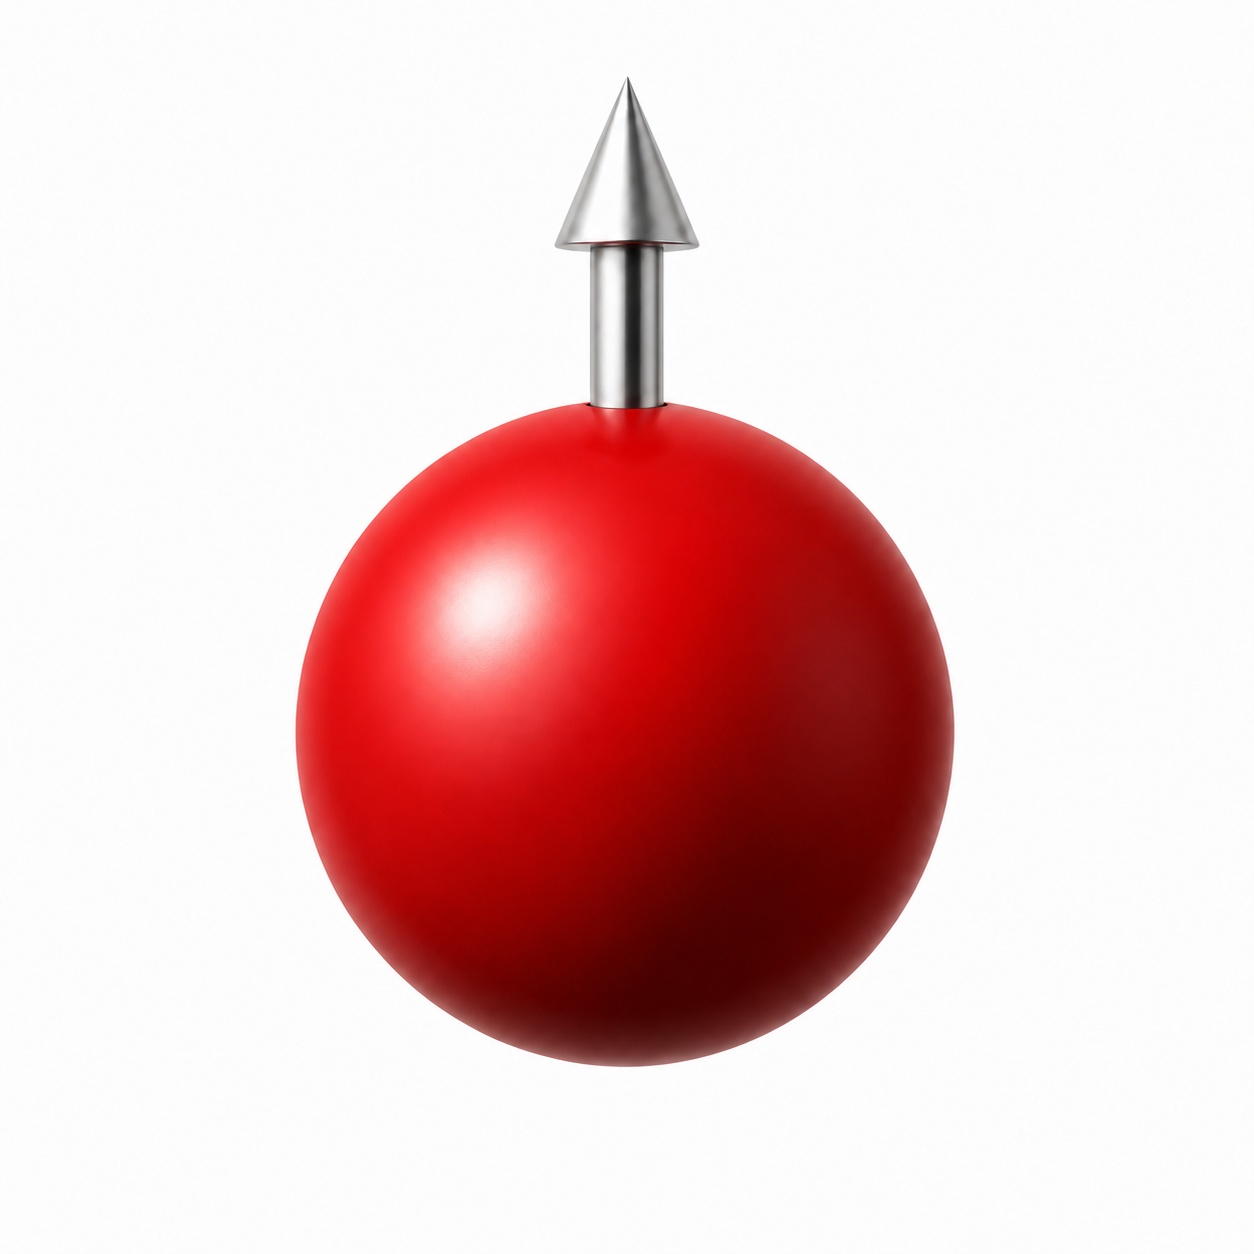
\includegraphics[width=0.6\textwidth]{assets/electron-arrow-up-v2.png}
        \\ \vspace{0.3cm}
        Spin-up: $\ket{1}$
    \end{minipage}
    \hfill
    \begin{minipage}{0.45\textwidth}
        \centering
        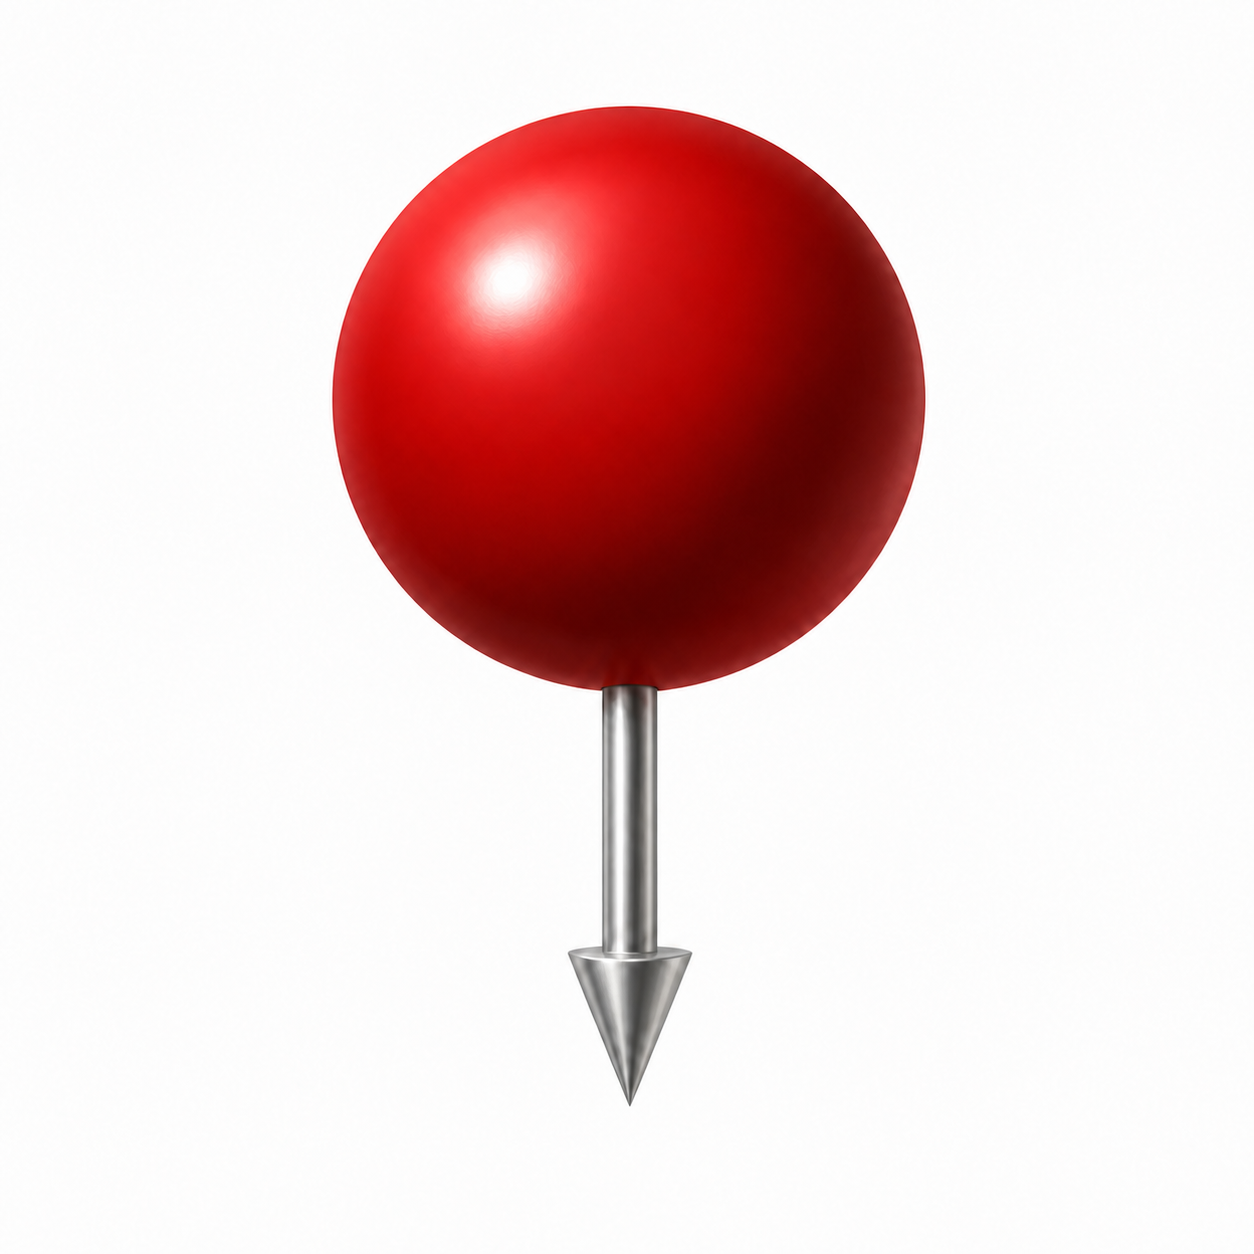
\includegraphics[width=0.6\textwidth]{assets/electron-arrow-down-v2.png}
        \\ \vspace{0.3cm}
        Spin-down: $\ket{0}$
    \end{minipage}
\end{figure}

But in contrast to classical bits, the electron's spin can also be in a
superposition of both up and down at once, meaning it's partly $\ket{0}$,
partly $\ket{1}$.

\begin{figure}[ht]
    \centering
    \begin{minipage}{0.4\textwidth}
        \centering
        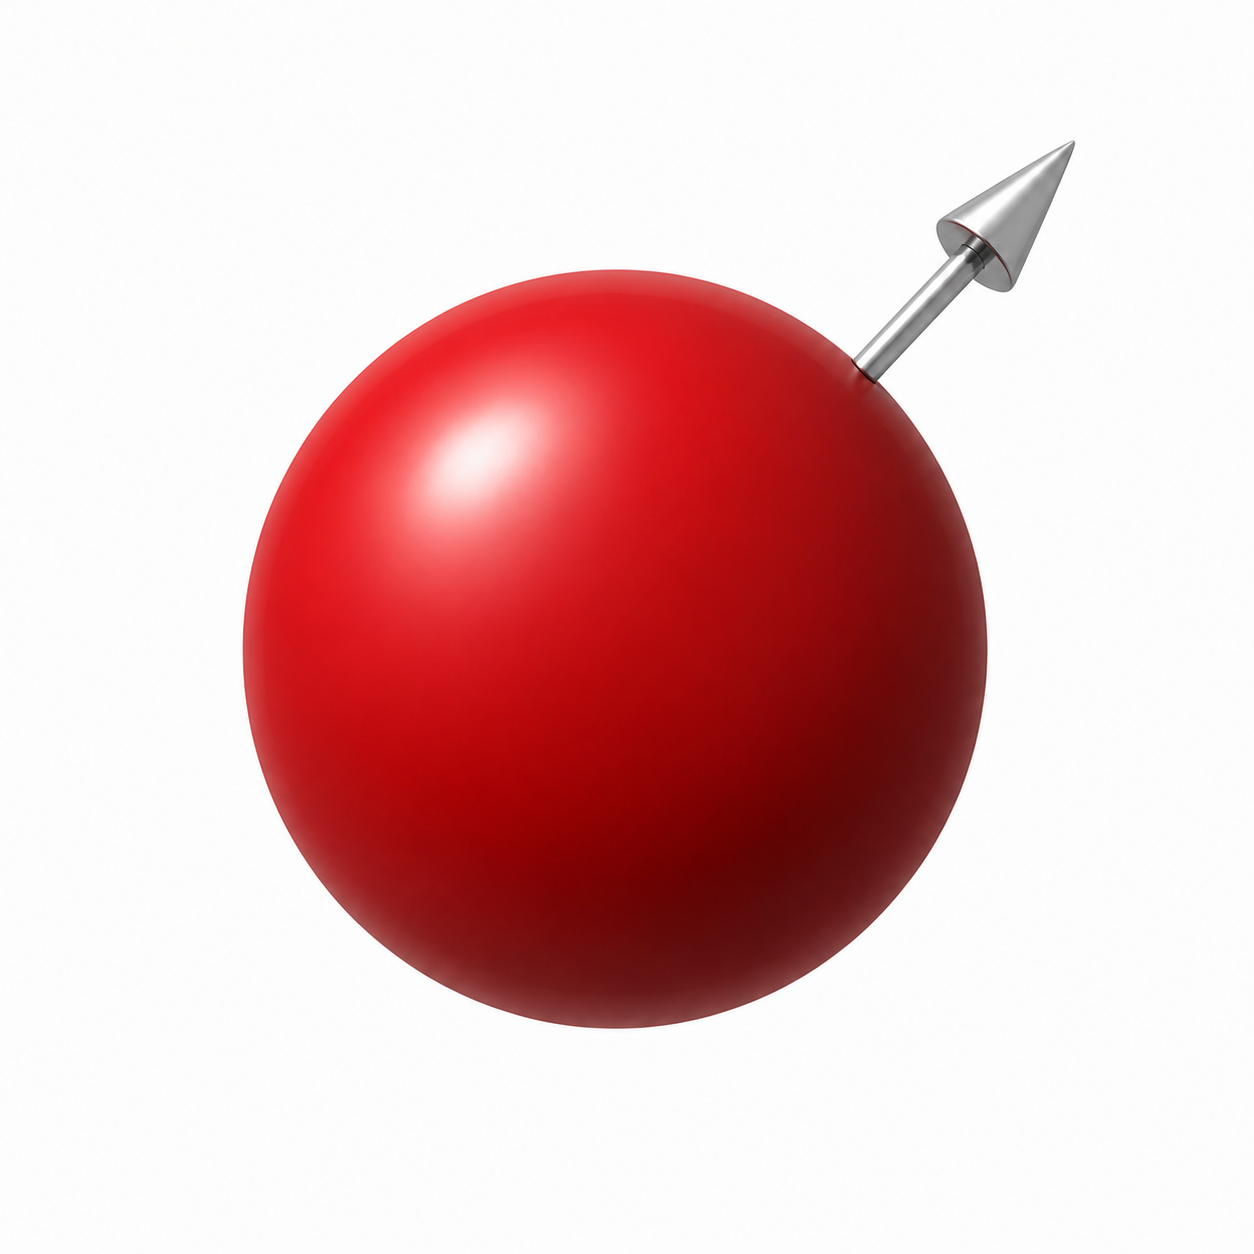
\includegraphics[width=0.6\textwidth]{assets/electron-arrow-diagonal-v2.png}
        \\ \vspace{0.3cm}
        Superposition: $\alpha\ket{0} + \beta\ket{1}$
    \end{minipage}
\end{figure}

This is what allows the qubit to behave fundamentally differently from a
classical bit and makes quantum computing possible.
Now that we have our foundations, we can move on to the interesting part.